\section{连续函数空间}
\label{sec:nspace-continuous-function-spaces}

连续函数是最接近一元分析经验的函数空间。本节先在紧度量空间上配以最大绝对值范数，证明它是Banach空间；再看定义域不紧时需要怎样调整；最后把同一个$C[0,1]$换成积分范数，看完备性怎样失去。

\paragraph{紧集上的一致范数}
设$K$是非空紧度量空间，$C(K)$为$K$上的全体$\mathbb K$值连续函数，在逐点运算下它是线性空间。定义
\begin{equation}
 \lVert f\rVert_\infty=\max_{x\in K}\lvert f(x)\rvert .
 \label{eq:nspace-uniform-norm}
\end{equation}
$\lvert f\rvert$是紧集上的实值连续函数，由第~\ref{chap:topological-spaces}章“紧集的连续像是紧集”，它的值域是$\mathbb R$中的紧集，所以最大值存在且有限。

这个范数称为\term{一致范数}（uniform norm），也称上确界范数。它的公理核验与上一节对$C[0,1]$的论证相同：在每个$x$处验证，再取最大值。当$K=\{1,\ldots,d\}$是有限集时，$C(K)$就是$\mathbb K^d$配最大分量范数，这正是函数作为向量的类比中最贴切的一个情形。

\paragraph{一致范数下的收敛}
$\lVert f_n-f\rVert_\infty\leq\varepsilon$意味着在所有$x\in K$处同时有$\lvert f_n(x)-f(x)\rvert\leq\varepsilon$，即$f_n$的整条曲线落在以$f$为中心、上下宽$\varepsilon$的带子里。所以一致范数下的收敛就是第~\ref{chap:metric-space-maps}章的一致收敛。

图~\ref{fig:nspace-uniform-tube}(a)是一个落在带内的例子。图~\ref{fig:nspace-uniform-tube}(b)中的$x^n$在$[0,1)$上逐点趋于$0$，但每条曲线都会在靠近$1$处越出零函数周围的带子，越出点随$n$右移却始终存在。

\begin{BookInlineFigure}
  \centering
  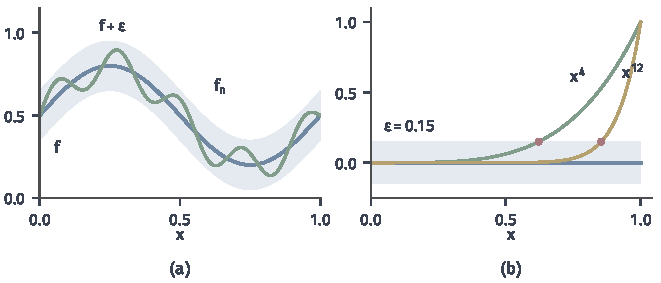
\includegraphics[width=112mm]{figures/04-spaces-measures-and-geometry/03-function-spaces/matplotlib/nspace-uniform-tube/figure.pdf}
  \caption{一致范数的几何意义，浅蓝色为半宽$\varepsilon=0.15$的带子。(a)$f(x)=0.5+0.3\sin(2\pi x)$（蓝）周围的带子，$f_n=f+0.1\sin(9\pi x)$（绿）整条曲线都在带内，所以$\lVert f_n-f\rVert_\infty=0.1$。(b)零函数周围的带子；$x^4$与$x^{12}$分别在红点$x=0.15^{1/4}$和$x=0.15^{1/12}$处越出带子。}
  \label{fig:nspace-uniform-tube}
\end{BookInlineFigure}

$x^n$在这个范数下连柯西列都不是。令$t=x^n$，当$x$跑遍$[0,1]$时$t$也跑遍$[0,1]$，所以
\[
 \lVert x^n-x^{2n}\rVert_\infty=\max_{t\in[0,1]}(t-t^2)=\frac14,
\]
这个值不随$n$减小。

\paragraph{完备性}
第~\ref{chap:metric-space-maps}章已经为一致收敛建立了两个结论：目标空间完备时，一致柯西的映射列一致收敛到某个映射；连续映射列的一致极限仍连续。$\mathbb K$是完备的，把两者合起来，就得到连续函数空间的完备性。

\begin{theorem}[紧集上连续函数空间的完备性]
\label{thm:nspace-ck-complete}
设$K$是非空紧度量空间。则$(C(K),\lVert\cdot\rVert_\infty)$是Banach空间。
\end{theorem}

\begin{proof}
设$(f_n)$是$C(K)$中的柯西列。对每个$\varepsilon>0$，存在$N$，使$m,n\geq N$时
\[
 \max_{x\in K}\lvert f_n(x)-f_m(x)\rvert<\varepsilon,
\]
这正说明$(f_n)$作为映射列是一致柯西的。

$\mathbb K$完备，所以$f_n$一致收敛到某个函数$f:K\to\mathbb K$。各$f_n$连续，一致极限$f$也连续，于是$f\in C(K)$。一致收敛就是$\lVert f_n-f\rVert_\infty\to0$，所以柯西列在$C(K)$中收敛。
\end{proof}

证明中三件事各有出处：候选极限由$\mathbb K$的完备性逐点给出；共同的误差阈值把逐点收敛加强为一致收敛；一致收敛保证极限连续。$K$的紧性只用来保证最大值有限，使式~\eqref{eq:nspace-uniform-norm}是范数。

\paragraph{非紧定义域}
在非紧的度量空间$X$上，连续函数可能无界，例如$\mathbb R$上的$f(x)=x$，一致“范数”不再是实数。这时只保留有界的连续函数，并把最大值换成上确界：
\begin{equation}
 C_b(X)=\Bigl\{f:X\to\mathbb K\ \text{连续}:\ \sup_{x\in X}\lvert f(x)\rvert<\infty\Bigr\},
 \label{eq:nspace-cb}
\end{equation}
范数为
\[
 \lVert f\rVert_\infty=\sup_{x\in X}\lvert f(x)\rvert.
\]
有界函数之和与数乘仍有界，所以$C_b(X)$是线性空间。

定理~\ref{thm:nspace-ck-complete}的证明中，候选极限的存在和连续都没有用到紧性。非紧时只需补充一步：一致极限仍然有界。取$N$使$n\geq N$时$\sup_x\lvert f_n(x)-f(x)\rvert\leq1$，则对每个$x$，
\[
 \lvert f(x)\rvert\leq\lvert f_N(x)\rvert+1\leq\lVert f_N\rVert_\infty+1,
\]
右边与$x$无关。于是$f\in C_b(X)$，所以$(C_b(X),\lVert\cdot\rVert_\infty)$对任意度量空间$X$都是Banach空间。

非紧定义域上会出现紧区间上没有的现象。在$C_b(\mathbb R)$中取移动的三角形
\[
 f_n(x)=\max\bigl(0,\ 1-\lvert x-n\rvert\bigr).
\]
每个固定的$x$在$n>\lvert x\rvert+1$以后都有$f_n(x)=0$，所以$f_n$逐点趋于零；但峰高始终为$1$，$\lVert f_n\rVert_\infty=1$，序列不依范数收敛。质量没有消失，只是移向无穷远，这与向量的单位列$e_n$的情形相同。

\paragraph{积分范数下的不完备}
回到$C[0,1]$，改用积分范数$\lVert f\rVert_1=\int_0^1\lvert f(x)\rvert\,dx$，其中积分对Lebesgue测度取，连续函数的Lebesgue积分与黎曼积分相同。集合没有变，只换了衡量误差的方式，完备性却会失去。

对$n\geq2$，令
\[
 g_n(x)=\begin{cases}0,&0\leq x\leq\frac12,\\ n\bigl(x-\frac12\bigr),&\frac12<x<\frac12+\frac1n,\\ 1,&\frac12+\frac1n\leq x\leq1.\end{cases}
\]
每个$g_n$连续，越来越陡地从$0$升到$1$，像是在逼近$\tfrac12$处跳跃的阶跃函数$\mathbf 1_{(1/2,1]}$，如图~\ref{fig:nspace-step-ramp}(a)所示。

\begin{BookInlineFigure}
  \centering
  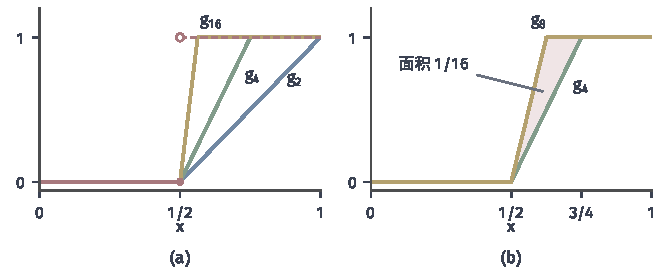
\includegraphics[width=112mm]{figures/04-spaces-measures-and-geometry/03-function-spaces/matplotlib/nspace-step-ramp/figure.pdf}
  \caption{积分范数下的柯西列。(a)折线$g_2,g_4,g_{16}$（蓝、绿、黄）越来越陡，红线是它们的积分极限$\mathbf 1_{(1/2,1]}$，空心圈表示跳跃。(b)$g_4$与$g_8$之间的浅红区域面积为$\lVert g_4-g_8\rVert_1=\tfrac1{16}$。}
  \label{fig:nspace-step-ramp}
\end{BookInlineFigure}

先算这列函数彼此的距离。设$m>n\geq2$，则$g_m\geq g_n$处处成立，所以
\[
 \lVert g_n-g_m\rVert_1=\int_0^1g_m\,dx-\int_0^1g_n\,dx.
\]
$g_n$下方的面积由一个底$\tfrac1n$、高$1$的三角形和宽$\tfrac12-\tfrac1n$的矩形组成，于是
\[
 \int_0^1g_n\,dx=\frac12-\frac1{2n}.
\]
代回前式，得到
\begin{equation}
 \lVert g_n-g_m\rVert_1=\frac1{2n}-\frac1{2m}.
 \label{eq:nspace-ramp-distance}
\end{equation}
例如$n=4$、$m=8$时距离是$\tfrac18-\tfrac1{16}=\tfrac1{16}$，就是图~\ref{fig:nspace-step-ramp}(b)中的面积。式~\eqref{eq:nspace-ramp-distance}小于$\tfrac1{2n}$，随$n$增大趋于零，所以$(g_n)$是柯西列。

下面证明它在$C[0,1]$中没有极限。假设存在$g\in C[0,1]$使$\lVert g_n-g\rVert_1\to0$。每个$g_n$在$[0,\tfrac12]$上为零，所以
\[
 \int_0^{1/2}\lvert g(x)\rvert\,dx\leq\int_0^1\lvert g_n(x)-g(x)\rvert\,dx\to0.
\]
左边不依赖$n$，只能为零；$\lvert g\rvert$连续且非负，故$g=0$在$[0,\tfrac12]$上处处成立。

再任取$\delta\in(0,\tfrac12)$。当$n>1/\delta$时，$g_n$在$[\tfrac12+\delta,1]$上恒为$1$，同样的论证给出
\[
 \int_{1/2+\delta}^1\lvert1-g(x)\rvert\,dx=0,
\]
所以$g=1$在$[\tfrac12+\delta,1]$上成立。$\delta$任意，所以$g$在$(\tfrac12,1]$上恒为$1$。于是$g(\tfrac12)=0$，而右侧极限为$1$，$g$在$\tfrac12$处不连续，矛盾。

所以$(C[0,1],\lVert\cdot\rVert_1)$不是Banach空间。同一列函数在一致范数下连柯西列都不是：取$x=\tfrac12+\tfrac1{2n}$，
\[
 \lvert g_{2n}(x)-g_n(x)\rvert=1-\frac12=\frac12.
\]

积分误差所指向的“极限”是阶跃函数，它不在连续函数之中，而且它在$\tfrac12$处取什么值并不影响积分。要让这样的极限有处可去，下一节把成员扩大为可测函数，并把几乎处处相等的函数看作同一个元素。
